\documentclass[tikz,border=8pt]{standalone}
\usepackage{tikz}
\usetikzlibrary{shapes.geometric,arrows.meta,positioning,calc,fit,backgrounds}
\usepackage[T1]{fontenc}
\usepackage{helvet}\renewcommand{\familydefault}{\sfdefault}

% pastel palette
\definecolor{bandA}{HTML}{EAF2FD}  % evidence gathering band
\definecolor{bandB}{HTML}{F3EEFB}  % distillation band
\definecolor{bandC}{HTML}{EAF7EF}  % application band
\definecolor{boxblue}{HTML}{C7DCF8}
\definecolor{boxpurple}{HTML}{DCD3F2}
\definecolor{boxgreen}{HTML}{C9E8D4}
\definecolor{chipadv}{HTML}{F8D0CE}
\definecolor{chipnat}{HTML}{FBE3C4}
\definecolor{chipben}{HTML}{D5EFC9}
\definecolor{dbcol}{HTML}{F5E6B8}
\definecolor{ink}{HTML}{2D3748}
\definecolor{arrowc}{HTML}{6B7280}

\tikzset{
  node distance=9mm and 11mm,
  every node/.style={font=\small, text=ink},
  box/.style={draw=ink!45, rounded corners=2.2mm, minimum height=9mm,
              minimum width=16mm, inner sep=2.4mm, line width=0.5pt},
  model/.style={box, fill=boxblue},
  modelp/.style={box, fill=boxpurple},
  modelg/.style={box, fill=boxgreen},
  chip/.style={draw=ink!35, rounded corners=1.6mm, inner sep=1.8mm,
               font=\footnotesize, line width=0.4pt},
  db/.style={cylinder, shape border rotate=90, draw=ink!45, fill=dbcol,
             aspect=0.14, minimum width=13mm, minimum height=11mm,
             inner sep=1.2mm, line width=0.5pt},
  arr/.style={-{Stealth[length=2.6mm]}, line width=0.7pt, draw=arrowc},
  lab/.style={font=\footnotesize, text=ink!80, inner sep=1pt},
  seclab/.style={font=\bfseries\small, text=ink},
}

\begin{document}
\begin{tikzpicture}

% ---------- Evidence Gathering (top, left -> right) ----------
\node[box, fill=white, align=center, inner sep=2.6mm] (task) at (0,0) {%
  \begin{tabular}{@{}c@{}}
  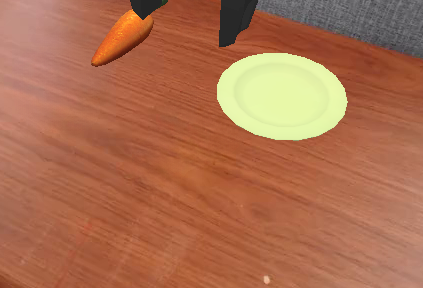
\includegraphics[width=17mm]{frames/method_frame.png}\\[1.2mm]
  {\footnotesize``put the carrot on the plate''}
  \end{tabular}};
\node[lab, above=0.8mm of task] {task \(=\) instruction \(+\) image};

\node[model, right=13mm of task] (vlm1) {VLM};

\node[chip, fill=chipnat, right=15mm of vlm1] (nat) {natural};
\node[chip, fill=chipadv, above=2.6mm of nat] (adv) {adversarial};
\node[chip, fill=chipben, below=2.6mm of nat] (ben) {benign};

\node[model, right=15mm of nat] (vla1) {VLA};
\node[db, right=13.5mm of vla1] (evidence) {\footnotesize evidence};

\draw[arr] (task) -- (vlm1);
\draw[arr] (vlm1) -- node[lab, above=0.4mm]{generate} node[lab, below=0.4mm]{rephrases} ($(nat.west)+(-1.5mm,0)$);
\draw[arr, shorten >=1mm] ($(vlm1.east)+(9mm,0)$) |- (adv.west);
\draw[arr, shorten >=1mm] ($(vlm1.east)+(9mm,0)$) |- (ben.west);
\draw[arr] (adv.east) -- ($(vla1.west)+(-1mm,1mm)$);
\draw[arr] (nat.east) -- (vla1.west);
\draw[arr] (ben.east) -- ($(vla1.west)+(-1mm,-1mm)$);
\draw[arr] (vla1) -- node[lab, above=0.4mm]{evaluate} node[lab, below=0.4mm]{(rollouts)} (evidence);

% ---------- Rule Distillation (right, top -> bottom) ----------
\node[modelp, below=11mm of evidence] (llm) {LLM};
\node[db, below=10mm of llm] (rules) {\footnotesize rules};
\draw[arr] (evidence) -- (llm);
\draw[arr] (llm) -- node[lab, right=1mm]{distill} (rules);

% ---------- Rule Application (bottom, right -> left) ----------
\node[modelg, left=16mm of rules] (vlm2) {VLM};
\node[box, fill=white, left=14mm of vlm2, align=center] (reph) {\footnotesize rephrased task};
\node[model, left=14mm of reph] (vla2) {VLA};

\node[chip, fill=white, draw=ink!30, above=7mm of vlm2, font=\footnotesize] (task2)
  {task \(=\) instruction \(+\) image};

\draw[arr] (rules) -- (vlm2);
\draw[arr] (task2) -- (vlm2);
\draw[arr] (vlm2) -- node[lab, above=0.5mm]{rephrase} (reph);
\draw[arr] (reph) -- (vla2);

% ---------- section bands + labels ----------
\begin{scope}[on background layer]
  \node[fit=(task)(vlm1)(adv)(ben)(vla1)(evidence), rounded corners=3mm,
        fill=bandA, inner sep=4.5mm, yshift=1mm] (bandtop) {};
  \node[fit=(llm)(rules), rounded corners=3mm, fill=bandB,
        inner xsep=5mm, inner ysep=3.5mm] (bandright) {};
  \node[fit=(vlm2)(reph)(vla2)(task2), rounded corners=3mm, fill=bandC,
        inner sep=4mm] (bandbot) {};
\end{scope}

\node[seclab, anchor=south west] at ($(bandtop.north west)+(1mm,0.6mm)$)
  {\textcolor{ink}{1\;\;Evidence gathering}};
\node[seclab, anchor=west, rotate=-90] at ($(bandright.north east)+(2.6mm,-1mm)$)
  {2\;\;Rule distillation};
\node[seclab, anchor=north west] at ($(bandbot.south west)+(1mm,-0.8mm)$)
  {3\;\;Rule application};

\end{tikzpicture}
\end{document}
